\ifspanish

\question Se tiene un problema de clasificación binaria definido por las siguientes verosimilitudes:
$$p_{X|H}(x|0) = 2 \exp\left(-2x \right) \quad x>0$$
$$p_{X|H}(x|1) =1 \quad 0<x<1 $$ 
\begin{parts}
\part Obtenga el test de razón de verosimilitudes para un valor genérico del umbral $\eta$
$$\frac{p_{X|H}(x|1)}{p_{X|H}(x|0)} \dunodcero \eta$$
\part Calcule la probabilidad de falsa alarma y de pérdidas del decisor anterior en función de $\eta$
\part Represente la curva característica de operación del decisor e indique sobre la misma los puntos de trabajo de:
\begin{itemize}
\item El decisor de máxima verosimilitud
\item El decisor máximo a posteriori si $P_H(0)=2P_H(1)$
\item El decisor Neyman Pearson para $P_{FA}\leq 0.1$
\end{itemize}
\part Considere ahora el siguiente decisor de umbral sobre la observación $x$
$$x \dunodcero \eta_u$$

y obtenga su probabilidad de falsa alarma y de pérdidas en función de $\eta_u$
\part Represente la curva característica de operación del decisor de umbral anterior y compárela con la curva característica del decisor LRT. ¿Qué esquema de decisión (el obtenido mediante el LRT o mediante un test de umbral) presenta mejores prestaciones? Justifique su respuesta.
\end{parts}

\begin{solution}
\begin{parts}
\part $\left\lbrace  \begin{array}{ll} 
D=1: & \eta' < x < 1 \\
D=0: & 0 < x < \eta'  \quad {\rm y} \quad x>1 
\end{array} \right. $ \\
donde $\displaystyle \eta'=\frac{1}{2} \ln 2 \eta$ y $\eta'>0$
\part $\displaystyle P_{\rm FA}=\left\lbrace \begin{array}{ll} \exp(-2\eta') -\exp(-2) &   0<\eta'<1 \\ 0 &  \eta'>1 \end{array} \quad \right.  \quad P_{\rm M}=\left\lbrace \begin{array}{ll} \eta' &  0<\eta'<1 \\ 1 &  \eta'>1 \end{array} \right. $
\part $ $ \\
\begin{tabular}{ll}
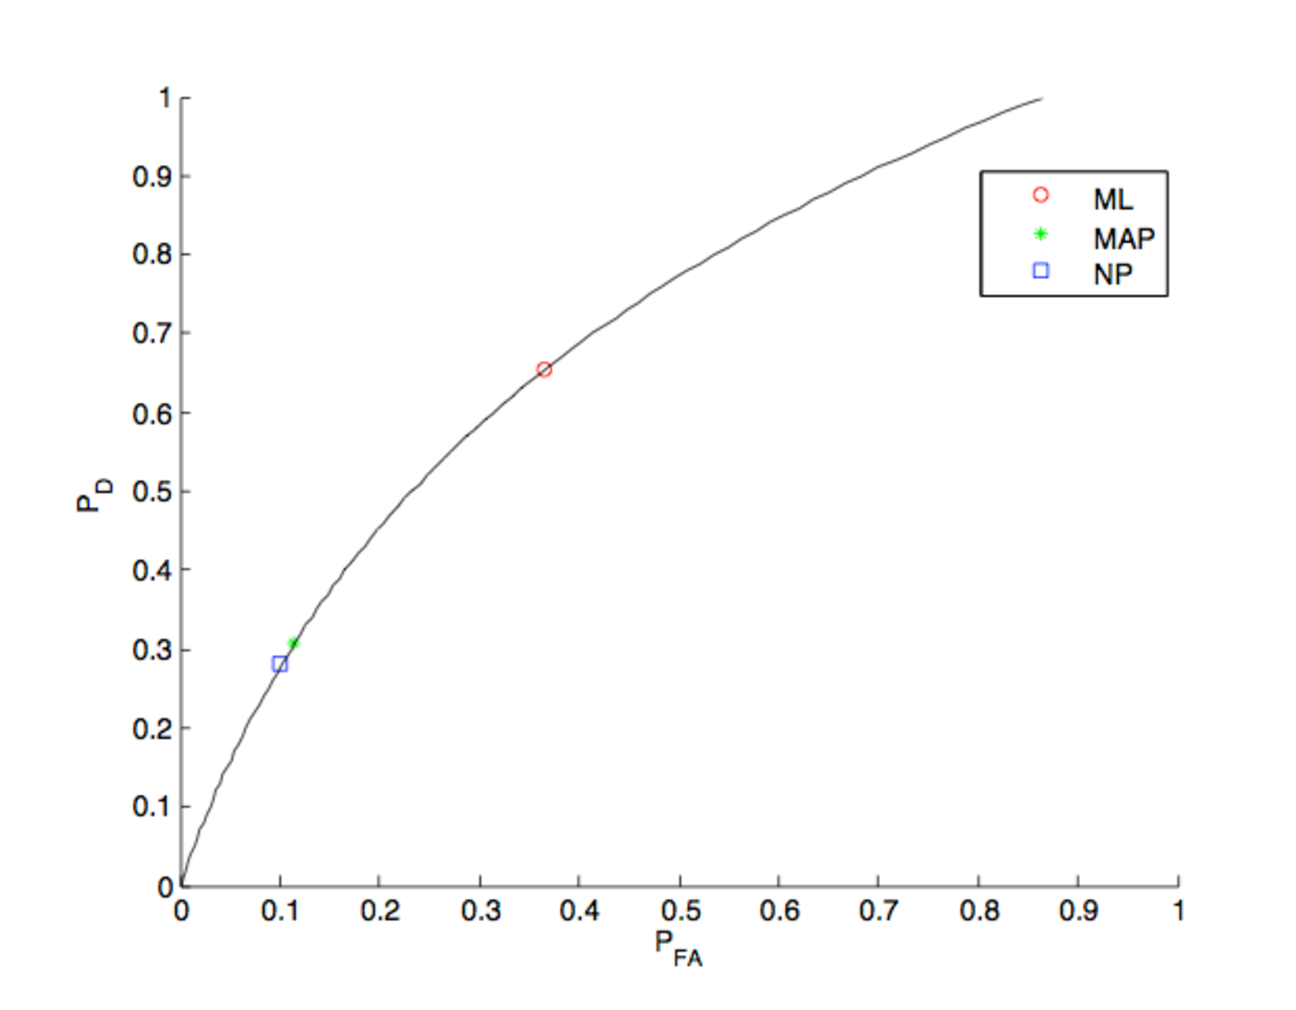
\includegraphics[width=5cm]{Figuras/ROC_jun2010_a.pdf} & 
$ \displaystyle  \begin{array}{lll} {\rm ML:}&  P_{\rm FA}= \frac{1}{2} -\exp(-2)  &  P_D=1-\frac{1}{2} \ln2 \\  {\rm MAP:}&  P_{\rm FA}= \frac{1}{4} -\exp(-2)  &  P_D=1- \ln2 \\ 
 {\rm N-P:}&  P_{\rm FA}= 0.1  \end{array} $
\end{tabular}
\part 
$\displaystyle P_{\rm FA}=\exp(-2\eta_u)\quad  \quad P_{\rm M}=\left\lbrace \begin{array}{ll} \eta_u&  0<\eta_u<1 \\ 1 &  \eta_u>1 \end{array} \right. $

\part $ $ \\
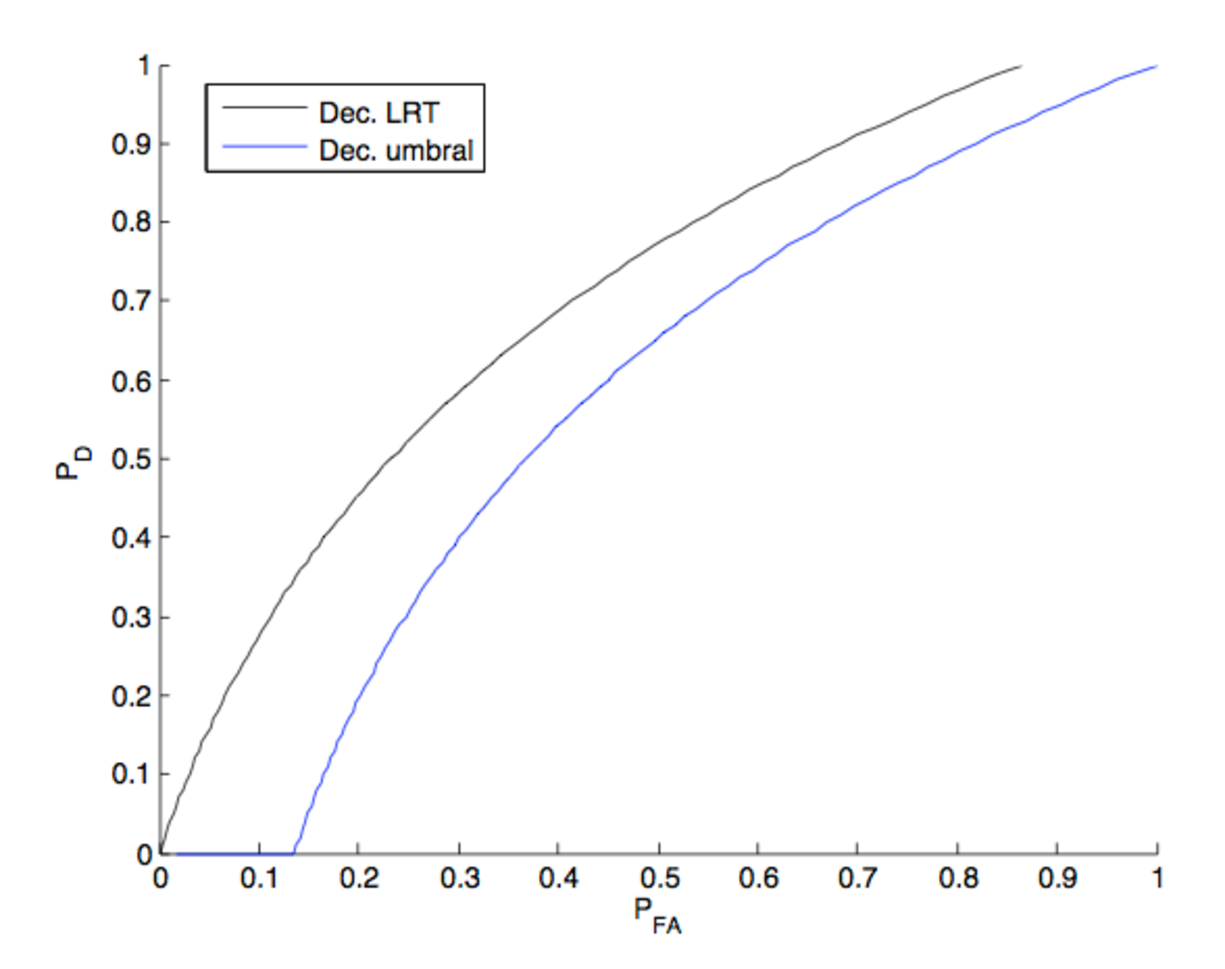
\includegraphics[width=5cm]{Figuras/ROC_jun2010_b.pdf}\\
Como era de esperar la curva ROC del decisor LRT está por encima de la ROC del decisor de umbral, por lo que confirmamos que el decisor LRT presenta mejores prestaciones.
\end{parts}

\end{solution}

\else

\question Consider a binary decision problem characterized by the following likelihoods:
$$p_{X|H}(x|0) = 2 \exp\left(-2x \right) \quad x>0$$
$$p_{X|H}(x|1) =1 \quad 0<x<1 $$ 
\begin{parts}
\part Obtain the likelihood ratio test for a generic value of threshold $\eta$.
$$\frac{p_{X|H}(x|1)}{p_{X|H}(x|0)} \begin{array}{c} {\scriptsize{D=1}} \\ \gtrless \\ {\scriptsize{D=0}}\end{array} \eta$$
\part Calculate the false alarm and missing probabilities of the previous decision maker as a function of $\eta$.
\part Plot the operating characteristic curve (ROC) of the decision maker, indicating in your representation the operation points of:
\begin{itemize}
\item The maximum likelihood decision maker
\item The maximum {\em a posteriori} decision maker, for $P_H(0)=2P_H(1)$
\item The Neyman-Pearson detector with $P_{FA}\leq 0.1$
\end{itemize}
\part Consider now a second decision maker consisting on imposing a threshold on the observation $x$
$$x \begin{array}{c} {\scriptsize{D=1}} \\ \gtrless \\ {\scriptsize{D=0}}\end{array} \eta_u$$
Obtain the false alarm and missing probabilities of this classifier as a function of $\eta_u$.
\part Plot the ROC of the new decision maker, and compare it with the ROC of the LRT decision maker. Which decision scheme (the one based on the LRT or the one based on a threshold over $x$) offers a better performance? Justify your answer.
\end{parts}

\begin{solution}
\begin{parts}
\part $\left\lbrace  \begin{array}{ll} 
D=1: & \eta' < x < 1 \\
D=0: & 0 < x < \eta'  \quad {\rm and} \quad x>1 
\end{array} \right. $ \\
where $\displaystyle \eta'=\frac{1}{2} \ln 2 \eta$ and $\eta'>0$
\part $\displaystyle P_{\rm FA}=\left\lbrace \begin{array}{ll} \exp(-2\eta') -\exp(-2) &   0<\eta'<1 \\ 0 &  \eta'>1 \end{array} \quad \right.  \quad P_{\rm M}=\left\lbrace \begin{array}{ll} \eta' &  0<\eta'<1 \\ 1 &  \eta'>1 \end{array} \right. $
\part $ $ \\
\begin{tabular}{ll}
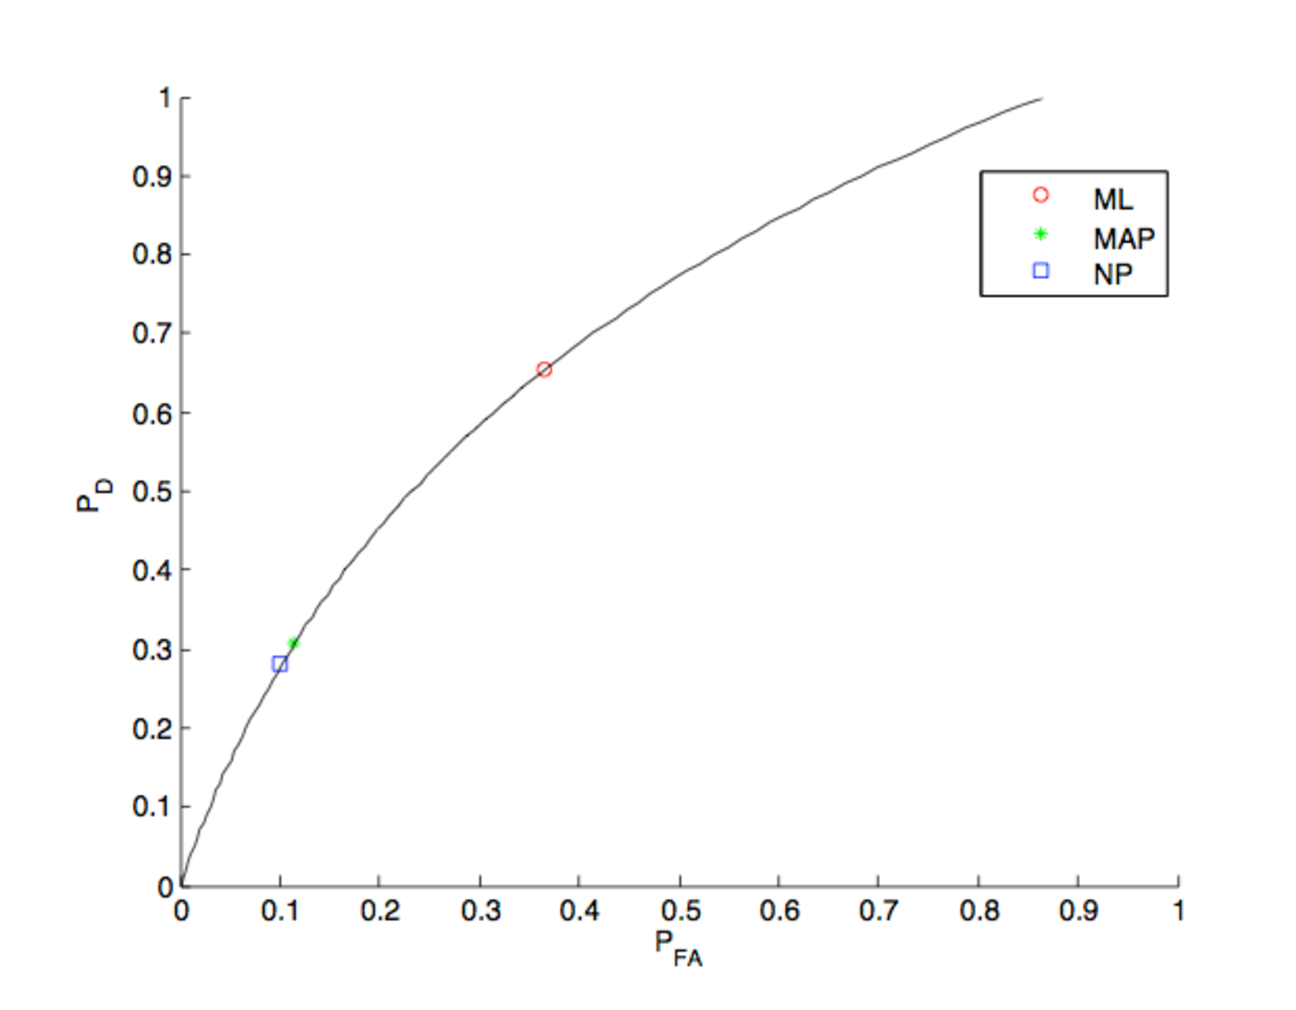
\includegraphics[width=5cm]{Figuras/ROC_jun2010_a.pdf} & 
$ \displaystyle  \begin{array}{lll} {\rm ML:}&  P_{\rm FA}= \frac{1}{2} -\exp(-2)  &  P_D=1-\frac{1}{2} \ln2 \\  {\rm MAP:}&  P_{\rm FA}= \frac{1}{4} -\exp(-2)  &  P_D=1- \ln2 \\ 
 {\rm N-P:}&  P_{\rm FA}= 0.1  \end{array} $
\end{tabular}
\part 
$\displaystyle P_{\rm FA}=\exp(-2\eta_u)\quad  \quad P_{\rm M}=\left\lbrace \begin{array}{ll} \eta_u&  0<\eta_u<1 \\ 1 &  \eta_u>1 \end{array} \right. $

\part $ $ \\
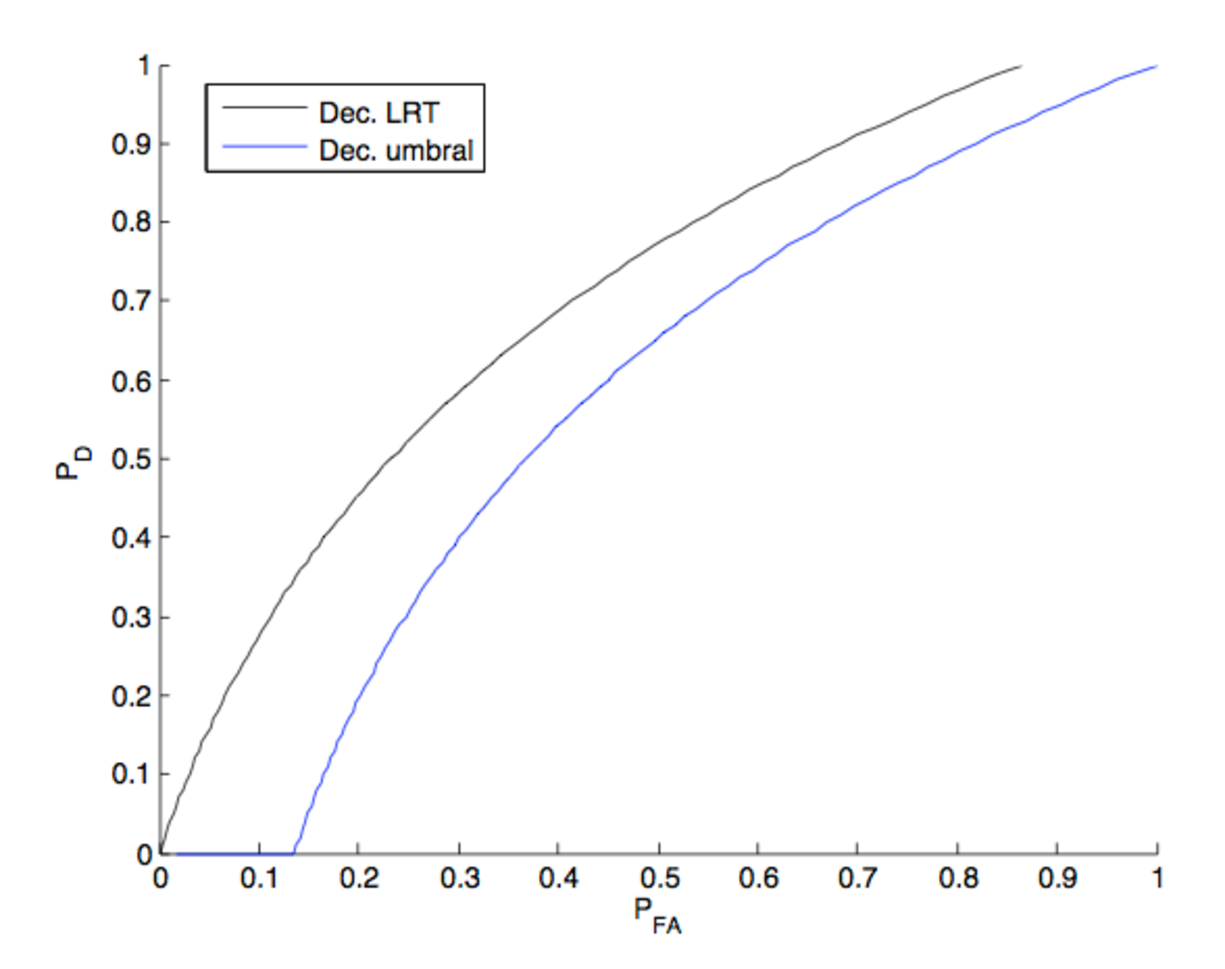
\includegraphics[width=5cm]{Figuras/ROC_jun2010_b.pdf}\\
As expected, the ROC corresponding to the LRT is above the ROC of the based on thresholding $x$; we confirm that the LRT decision makers achieve better performance.
\end{parts}

\end{solution}

\fi